\chapter{Sensitivity Estimate: Preliminary Results}\label{sensitivity}

\begin{figure}[h]
        \centering
        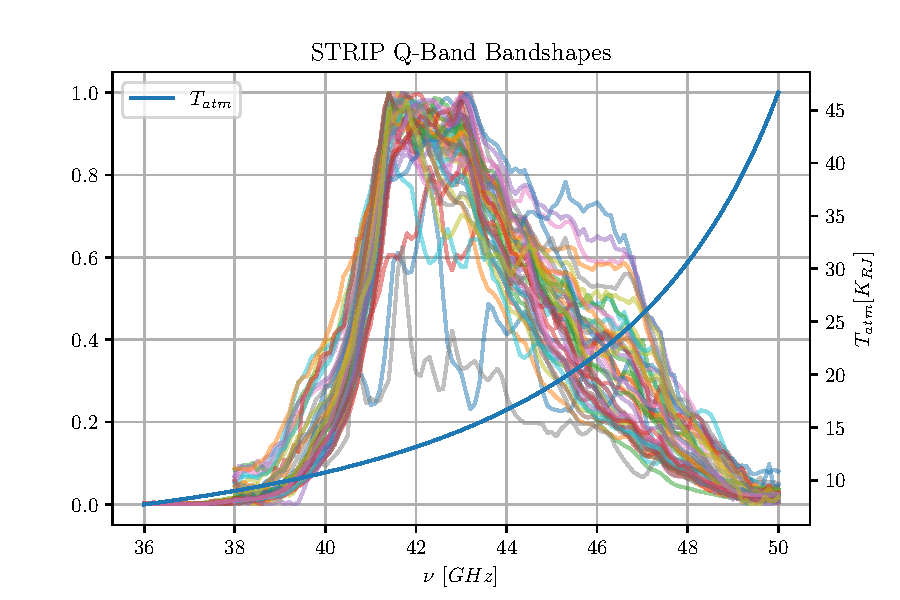
\includegraphics[width=\textwidth]{Strip_Bandshapes+TATM}
        \caption{Bandshapes of the Q-band detectors of the LSPE/Strip
        telescope. The blue curve represents the simulated atmopsheric
        brightness temperature as a function of frequency.}
        \label{fig:strip_bandshapes_tatm}
\end{figure}

\begin{figure}
        \centering
        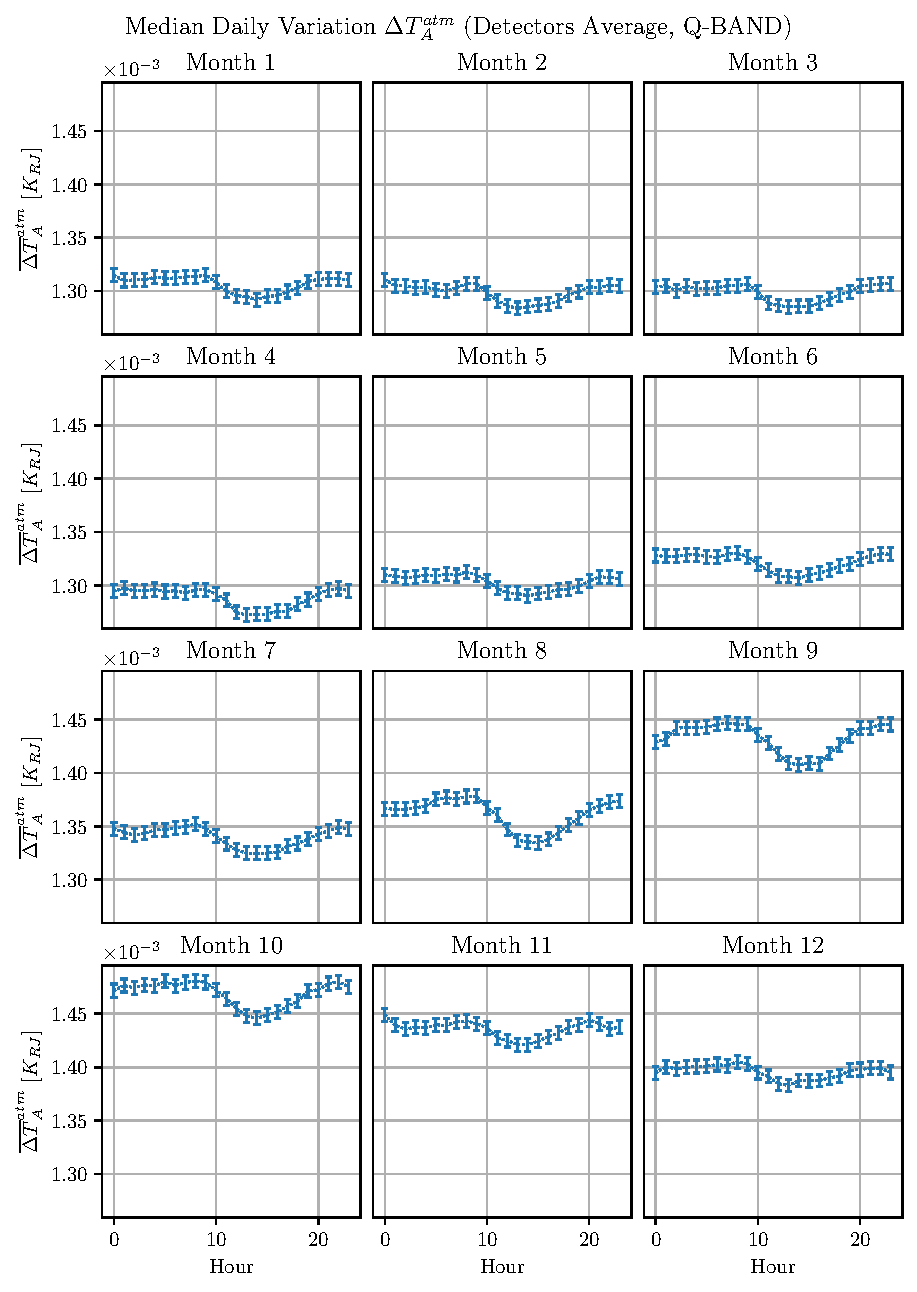
\includegraphics[width=0.96\textwidth]{TA_Sens_Detectors_Average_Teide}
        \caption{Seasonal variations of the maximum sensitivity reached by
        LSPE/Strip Q-band detectors. The reported values and the
        corresponding errors are obtained by averaging over the 49
        detectors.}
        \label{fig:ta_sens_detectors_average_teide}
\end{figure}

\begin{figure}
        \centering
        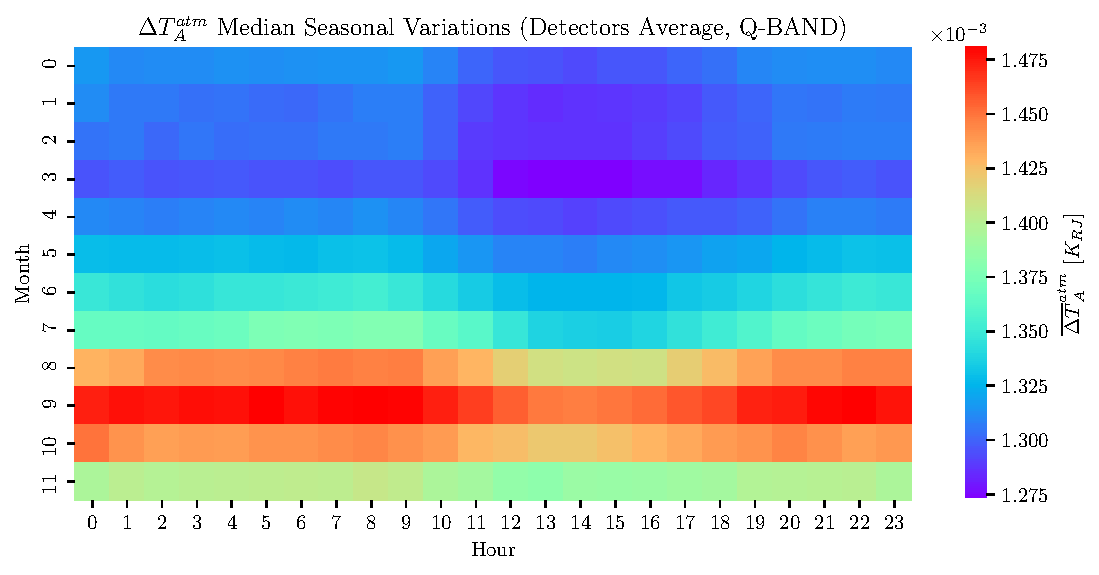
\includegraphics[width=\textwidth]{TA_Sens_Matrix_Detectors_Average}
        \caption{Color map representation of the seasonal variations of the
        maximum sensitivity reached by LSPE/Strip detectors, due to atmospheric
        effects.}
        \label{fig:ta_sens_matrix_detectors_average}
\end{figure}

